%%% LaTeX Template: Designer's CV
%%%
%%% Source: http://www.howtotex.com/
%%% Feel free to distribute this template, but please keep the referal to HowToTeX.com.
%%% Date: March 2012


%%%%%%%%%%%%%%%%%%%%%%%%%%%%%%%%%%%%%
% Document properties and packages
%%%%%%%%%%%%%%%%%%%%%%%%%%%%%%%%%%%%%
\documentclass[a4paper,12pt,final]{memoir}

% misc
\renewcommand{\familydefault}{bch}	% font
\pagestyle{empty}					% no pagenumbering
\setlength{\parindent}{0pt}			% no paragraph indentation


% required packages (add your own)
\usepackage{flowfram}										% column layout
\usepackage[top=1cm,left=1cm,right=1cm,bottom=1cm]{geometry}% margins
\usepackage{graphicx}										% figures
\usepackage{url}											% URLs
\usepackage[usenames,dvipsnames]{xcolor}					% color
\usepackage{multicol}										% columns env.
	\setlength{\multicolsep}{0pt}
\usepackage{paralist}										% compact lists
\usepackage{tikz}

%%%%%%%%%%%%%%%%%%%%%%%%%%%%%%%%%%%%%
% Create column layout
%%%%%%%%%%%%%%%%%%%%%%%%%%%%%%%%%%%%%
% define length commands
\setlength{\vcolumnsep}{\baselineskip}
\setlength{\columnsep}{\vcolumnsep}

% frame setup (flowfram package)
% left frame
\newflowframe{0.2\textwidth}{\textheight}{0pt}{0pt}[left]
	\newlength{\LeftMainSep}
	\setlength{\LeftMainSep}{0.2\textwidth}
	\addtolength{\LeftMainSep}{1\columnsep}
 
% small static frame for the vertical line
\newstaticframe{1.5pt}{\textheight}{\LeftMainSep}{0pt}
 
% content of the static frame
\begin{staticcontents}{1}
\hfill
\tikz{%
	\draw[loosely dotted,color=RoyalBlue,line width=1.5pt,yshift=0]
	(0,0) -- (0,\textheight);}%
\hfill\mbox{}
\end{staticcontents}
 
% right frame
\addtolength{\LeftMainSep}{1.5pt}
\addtolength{\LeftMainSep}{1\columnsep}
\newflowframe{0.7\textwidth}{\textheight}{\LeftMainSep}{0pt}[main01]


%%%%%%%%%%%%%%%%%%%%%%%%%%%%%%%%%%%%%
% define macros (for convience)
%%%%%%%%%%%%%%%%%%%%%%%%%%%%%%%%%%%%%
\newcommand{\Sep}{\vspace{1.5em}}
\newcommand{\SmallSep}{\vspace{0.5em}}

\newenvironment{AboutMe}
	{\ignorespaces\textbf{\color{RoyalBlue} About me}}
	{\Sep\ignorespacesafterend}
	
\newcommand{\CVSection}[1]
	{\Large\textbf{#1}\par
	\SmallSep\normalsize\normalfont}

\newcommand{\CVItem}[1]
	{\textbf{\color{RoyalBlue} #1}}

\usepackage{hyperref}
%%%%%%%%%%%%%%%%%%%%%%%%%%%%%%%%%%%%%
% Begin document
%%%%%%%%%%%%%%%%%%%%%%%%%%%%%%%%%%%%%
\begin{document}

% Left frame
%%%%%%%%%%%%%%%%%%%%
\begin{figure}
	\hfill
	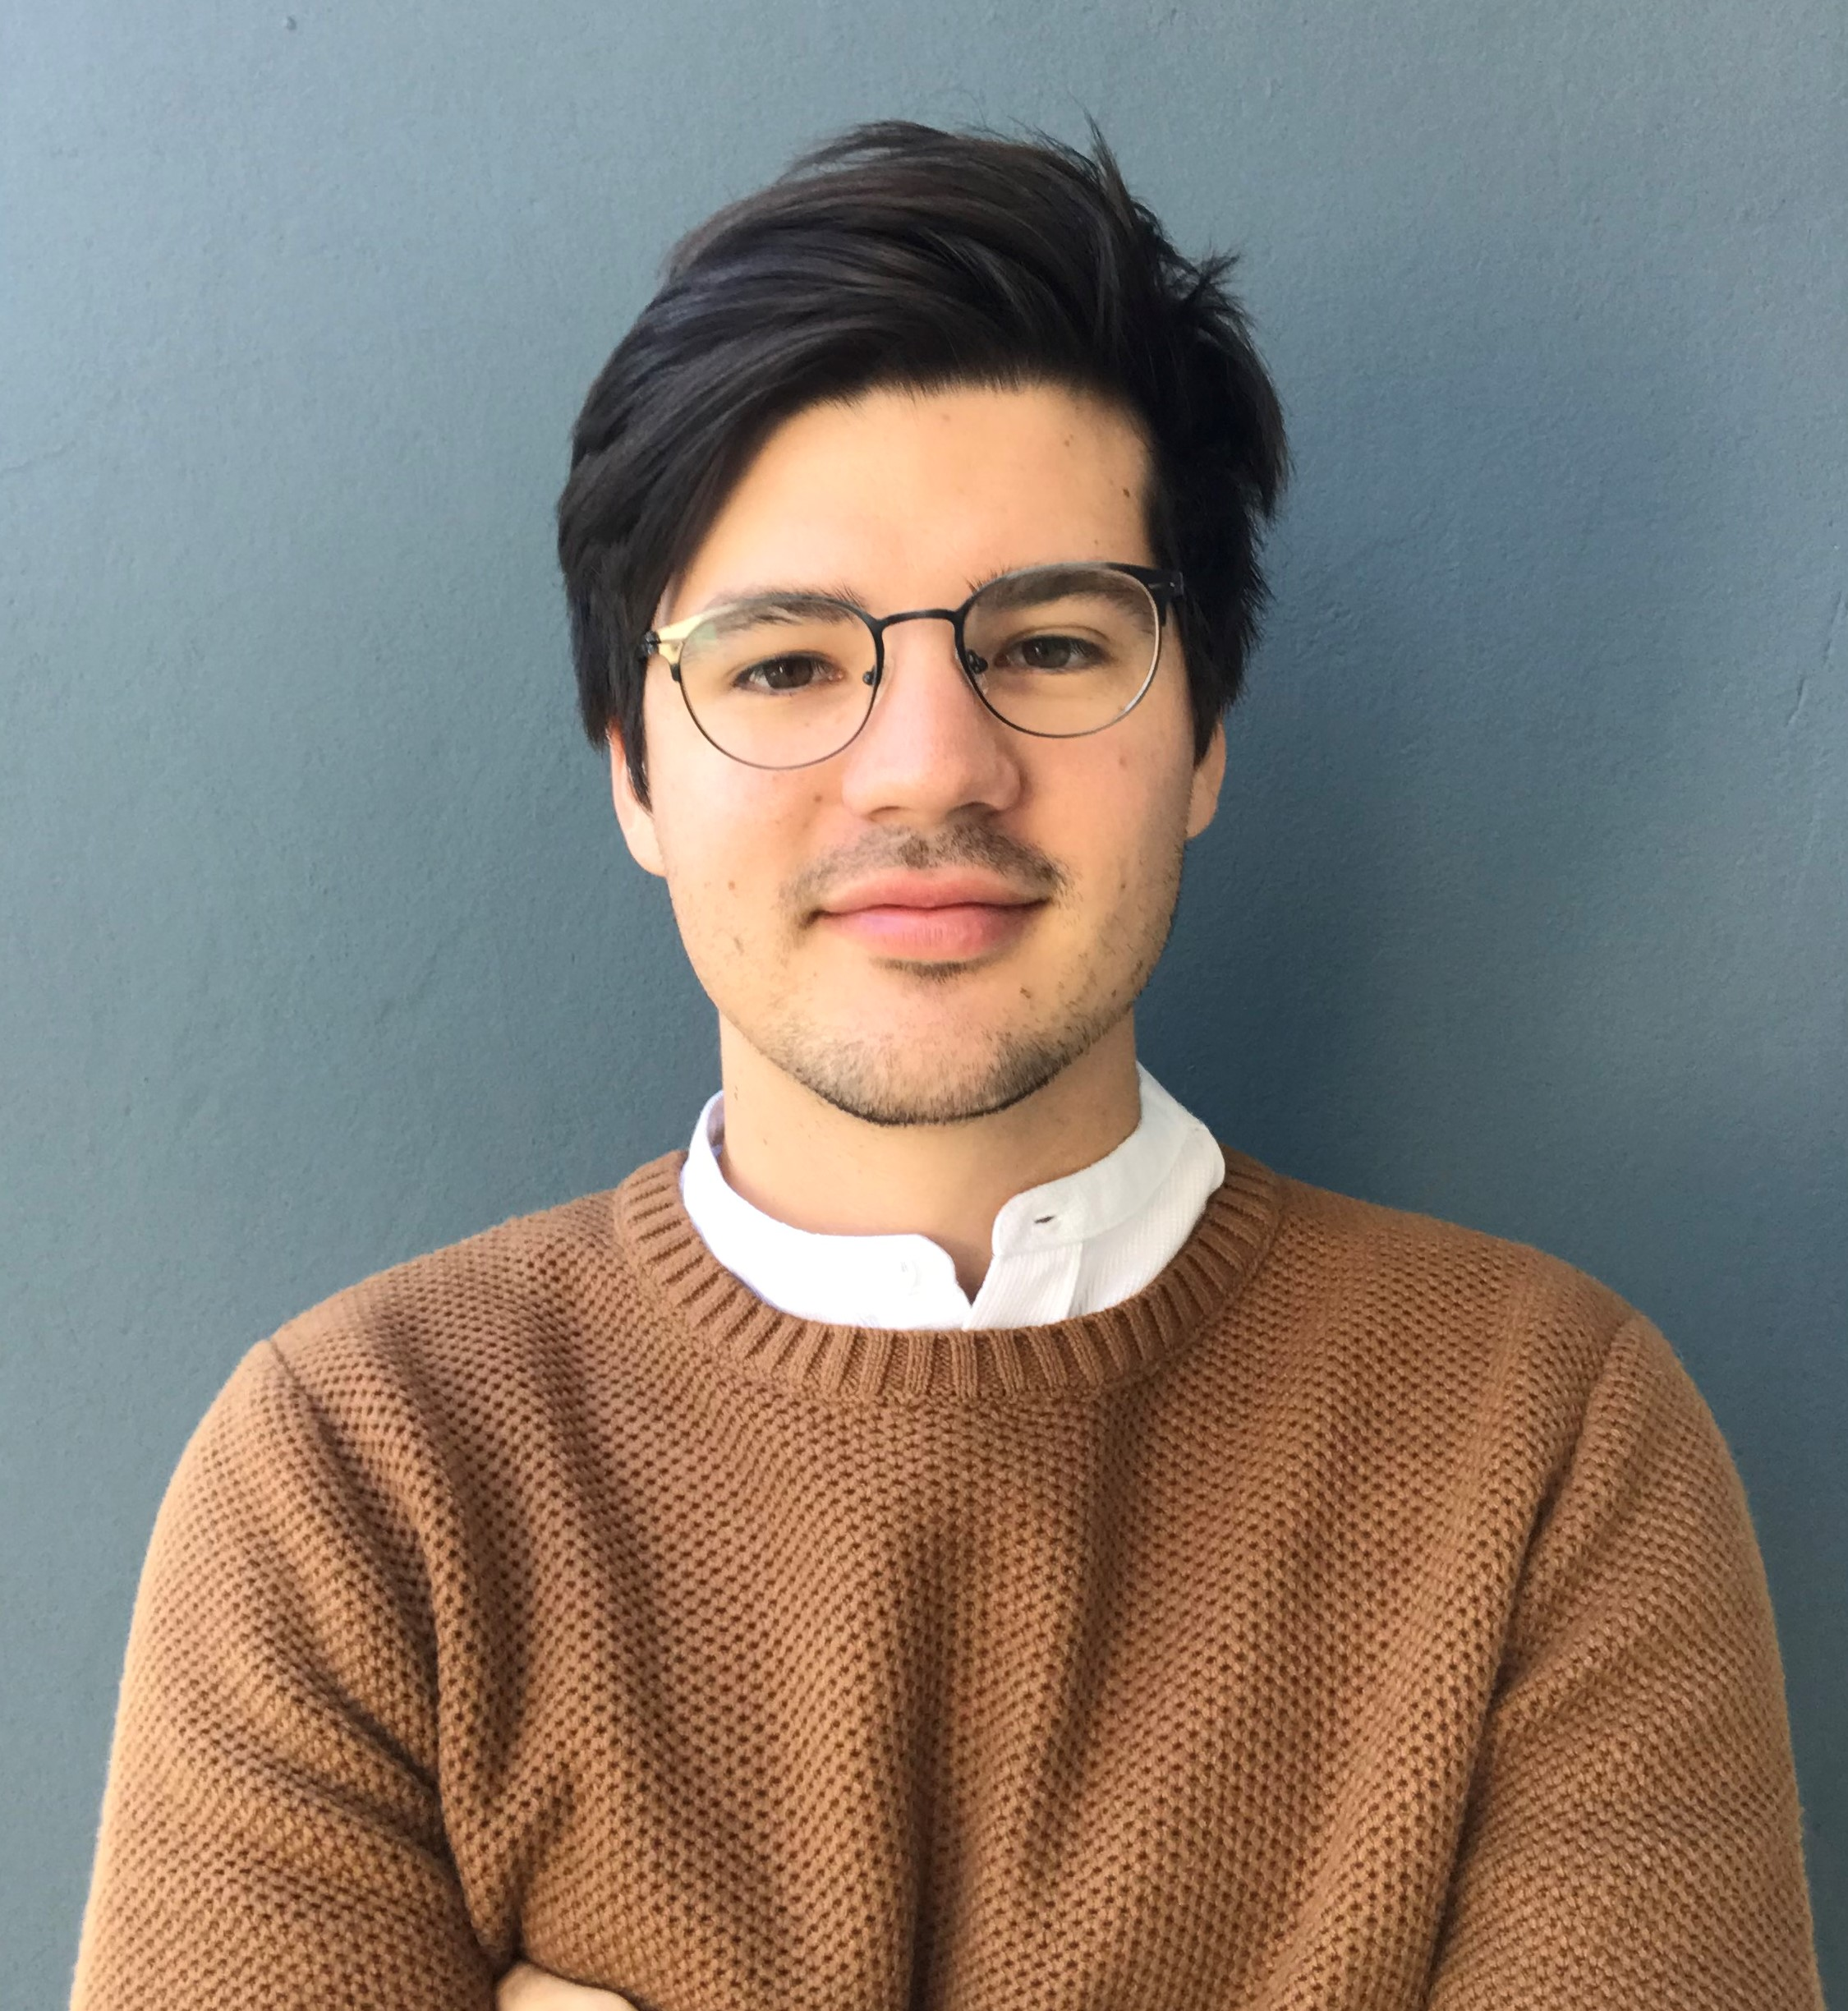
\includegraphics[width=0.7\columnwidth ]{picture}
	\vspace{-5cm}
\end{figure}


\begin{flushright}\small
	
	\CVItem{Chris Viviers}\\
	South African\\
	\vspace{0.5cm}	
	\CVItem{Current Residency}\\
	Rotterdam, Netherlands\\
	\vspace{0.5cm}
	\CVItem{Languages}\\
	English \\
	Afrikaans\\
	Dutch A1 \\
	\vspace{0.5cm}	
	\CVItem{Contact}\\	
	\href{mailto:ChrisViviers1@gmail.com}{ChrisViviers1@gmail}\\
	\href{http://www.omnitek-fus.com}{OmniTek-Fus.com}\\
	\href{https://www.facebook.com/christiaan.viviers.1}{fb://christiaan}\\
	\href{https://github.com/Chris-On-PC}{github:chris\_on\_pc}\\
	\href{https://www.linkedin.com/in/chrisviviers}{LinkedIn:chrisviviers}\\
	(+31) 62 066 0171
	
	
\end{flushright}\normalsize

\framebreak


% Right frame
%%%%%%%%%%%%%%%%%%%%
\Huge\bfseries {\color{RoyalBlue} Christiaan G$\ddot{u}$nter Alwyn Viviers} \\
\Large\bfseries  Electrical \& Electronic Engineer \\

\normalsize\normalfont

% About me
\begin{AboutMe}
As a technology enthusiast with a never-ending desire to learn new things, I believe that there is always work to be done. I am an ambitious and determined individual that enjoys the challenges that come with problem solving. By applying my unique perspective to approaching problems, I am able to bring about creative solutions. Regardless of the work that I am busy with, it is always driven by a passion for a positive impact on society.
\end{AboutMe}

% Experience
\CVSection{Experience}
\CVItem{Aug 2018 - Present, Software Engineer at Philips}\\
I joined Philips Image Guided Therapy systems (IGTs) as part of the system test team. My responsibilities are divided between working on improving test automation and the technologies my team has access to, as well as introducing various new software platforms to Philips IGTs.\\ \textbf{Best, Netherlands}.\SmallSep

\CVItem{June 2018 - Present, Engineering Trainee at Yacht}\\
I am a part of a program designed by Yacht to accelerate personal and technical growth. The goal is to develop specialist engineering skills through intercompany client projects while developing leadership, management and other soft skills through active coaching and guidance.\\ \textbf{Eindhoven, Netherlands.}\SmallSep

\CVItem{Feb 2016 - July 2017, Student Assistant}\\
I assisted in teaching various electric and electronic engineering-related courses at the University of Stellenbosch. Some of these include: C programming, Electronic Design and Electronic Components.\\ \textbf{Stellenbosch, South Africa.}\SmallSep

\CVItem{Jan 2016 - Mar 2016, Researcher}\\
Research and Development of Biosensors and Microfluidics at SAND microfluidic laboratory, Stellenbosch University. Successfully developed a biosensor prototype for bacteria detection.\\ \textbf{Stellenbosch, South Africa}
\SmallSep

% Education
\CVSection{Education}
\CVItem{2016 - 2017, MEng. Electrical \& Electronic}\\
Masters Degree (MEng.) Electrical \& Electronic Engineering. Cum Laude. Biotechnology Specialization. Thesis title: The Design and Fabrication of an Autophagy Flux Biosensor.\\ \textbf{Stellenbosch University, Western Cape, South Africa.} \SmallSep

\CVItem{2016 - 2019, Online Courses}\\
Various online courses completed

	\begin{compactitem}[\color{RoyalBlue}$\circ$]
		\item \href{https://www.coursera.org/account/accomplishments/certificate/AAHD8EMUXK8G}{Machine Learning}, Stanford University on Coursera, Andrew Ng 
		\item \href{https://confirm.udacity.com/DQXWUUCZ}{Full Stack Web Development Nanodegree}, Udacity
		\item \href{}{Secure \& Private AI}, Udacity
	\end{compactitem}

\SmallSep
\newpage
% Left frame
%%%%%%%%%%%%%%%%%%%%


\begin{flushright}\small
	
\end{flushright}\normalsize
\framebreak

\SmallSep
\CVItem{2012 - 2015, BEng. Electrical \& Electronic}\\
Bachelor Degree (BEng.) Electrical \& Electronic Engineering. Informatics Specialization. Thesis: Development of a Resistive Microfluidic Sensing Device for Pathogen Detection. Awarded the Jac Van der Merwe prize for the most innovative thesis in the Faculty of Engineering 2015.\\ \textbf{Stellenbosch University, Western Cape, South Africa.} \SmallSep 
\SmallSep

\CVItem{2007 - 2011, High School Diploma}\\
Graduated from High School at Oudtshoorn High School.\\ \textbf{Oudtshoorn, Western Cape, South Africa.}  
\SmallSep

% Skills
\CVSection{Skills \& Competences}


\CVItem{Programming Languages}
\begin{multicols}{3}
	\begin{compactitem}[\color{RoyalBlue}$\circ$]
		\item C\#
		\item Python 
		\item C/C++
		\item JavaScript
		\item MatLab/Octave
		\item HTML \& CSS
	\end{compactitem}
\end{multicols}
\SmallSep
\CVItem{Platforms}
\begin{multicols}{3}
	\begin{compactitem}[\color{RoyalBlue}$\circ$]
		\item Blender 
		\item Unity 3D
		\item Eagle
		\item AutoCAD: Inventor
		\item PTC Integrity	
		\item Unix
	\end{compactitem}
\end{multicols}
\SmallSep
\CVItem{Software Frameworks}
\begin{multicols}{3}
	\begin{compactitem}[\color{RoyalBlue}$\circ$]
		\item OpenCV 
		\item Tensorflow - Keras
		\item PyTorch
		\item Bootstrap
		\item .Net
		\item Git Version Control
	\end{compactitem}
\end{multicols}
\SmallSep
\CVItem{Other}
\begin{multicols}{3}
	\begin{compactitem}[\color{RoyalBlue}$\circ$]
		\item Critical Thinker
		\item Goal Orientated
		\item Team Work
		\item Strong Communication Skills
		\item Hardware Design 
		\item Antibody Work 
		\item Cell Culture
		\item Data Analytics
	\end{compactitem}
\end{multicols}
\Sep 
\CVSection{Hobbies \& Interests}
From an early age, I have always loved to analyze, dismantle and tinker with all kinds of gadgets and gizmos. The majority of my free time is spent exploring the latest tech that I can get my hands on or delving into a new piece of software that could open up exciting opportunities. Another passion of mine is traveling. As a curious mind, I am extremely captivated by what lies across the horizon, whether it be vast landscapes, interesting foods or a unique philosophy to live by. I am also a strong believer in learning new things through engaging with new cultures and working in different environments. At the end of a long day of eager learning, there is nothing quite as relaxing as indulging in the latest digital entertainment or spending quality time with friends and family.      

\Sep 
% References
\CVSection{References}

	\begin{compactitem}[\color{RoyalBlue}$\circ$]
		\item \CVItem{Prof WJ (Willem) Perold}\\Position: Vice Dean of research. Stellenbosch University Undergraduate and Masters degree Supervisor.\\Email: wjperold@sun.ac.za
		\item \CVItem{Prof Ben Loos}\\Position: Professor Stellenbosch University  Masters co-supervisor\\Email: bloos@sun.ac.za
	\end{compactitem}


%%%%%%%%%%%%%%%%%%%%%%%%%%%%%%%%%%%%%
% End document
%%%%%%%%%%%%%%%%%%%%%%%%%%%%%%%%%%%%%
\end{document}